\documentclass{standalone}
\usepackage{tikz}
\usetikzlibrary{patterns}
\usetikzlibrary{positioning}
\usetikzlibrary{patterns, positioning}
\usetikzlibrary{shapes.misc}
\usepackage[outline]{contour}
\contourlength{1.5pt} 
\usepackage[sfdefault]{ClearSans}

\begin{document}
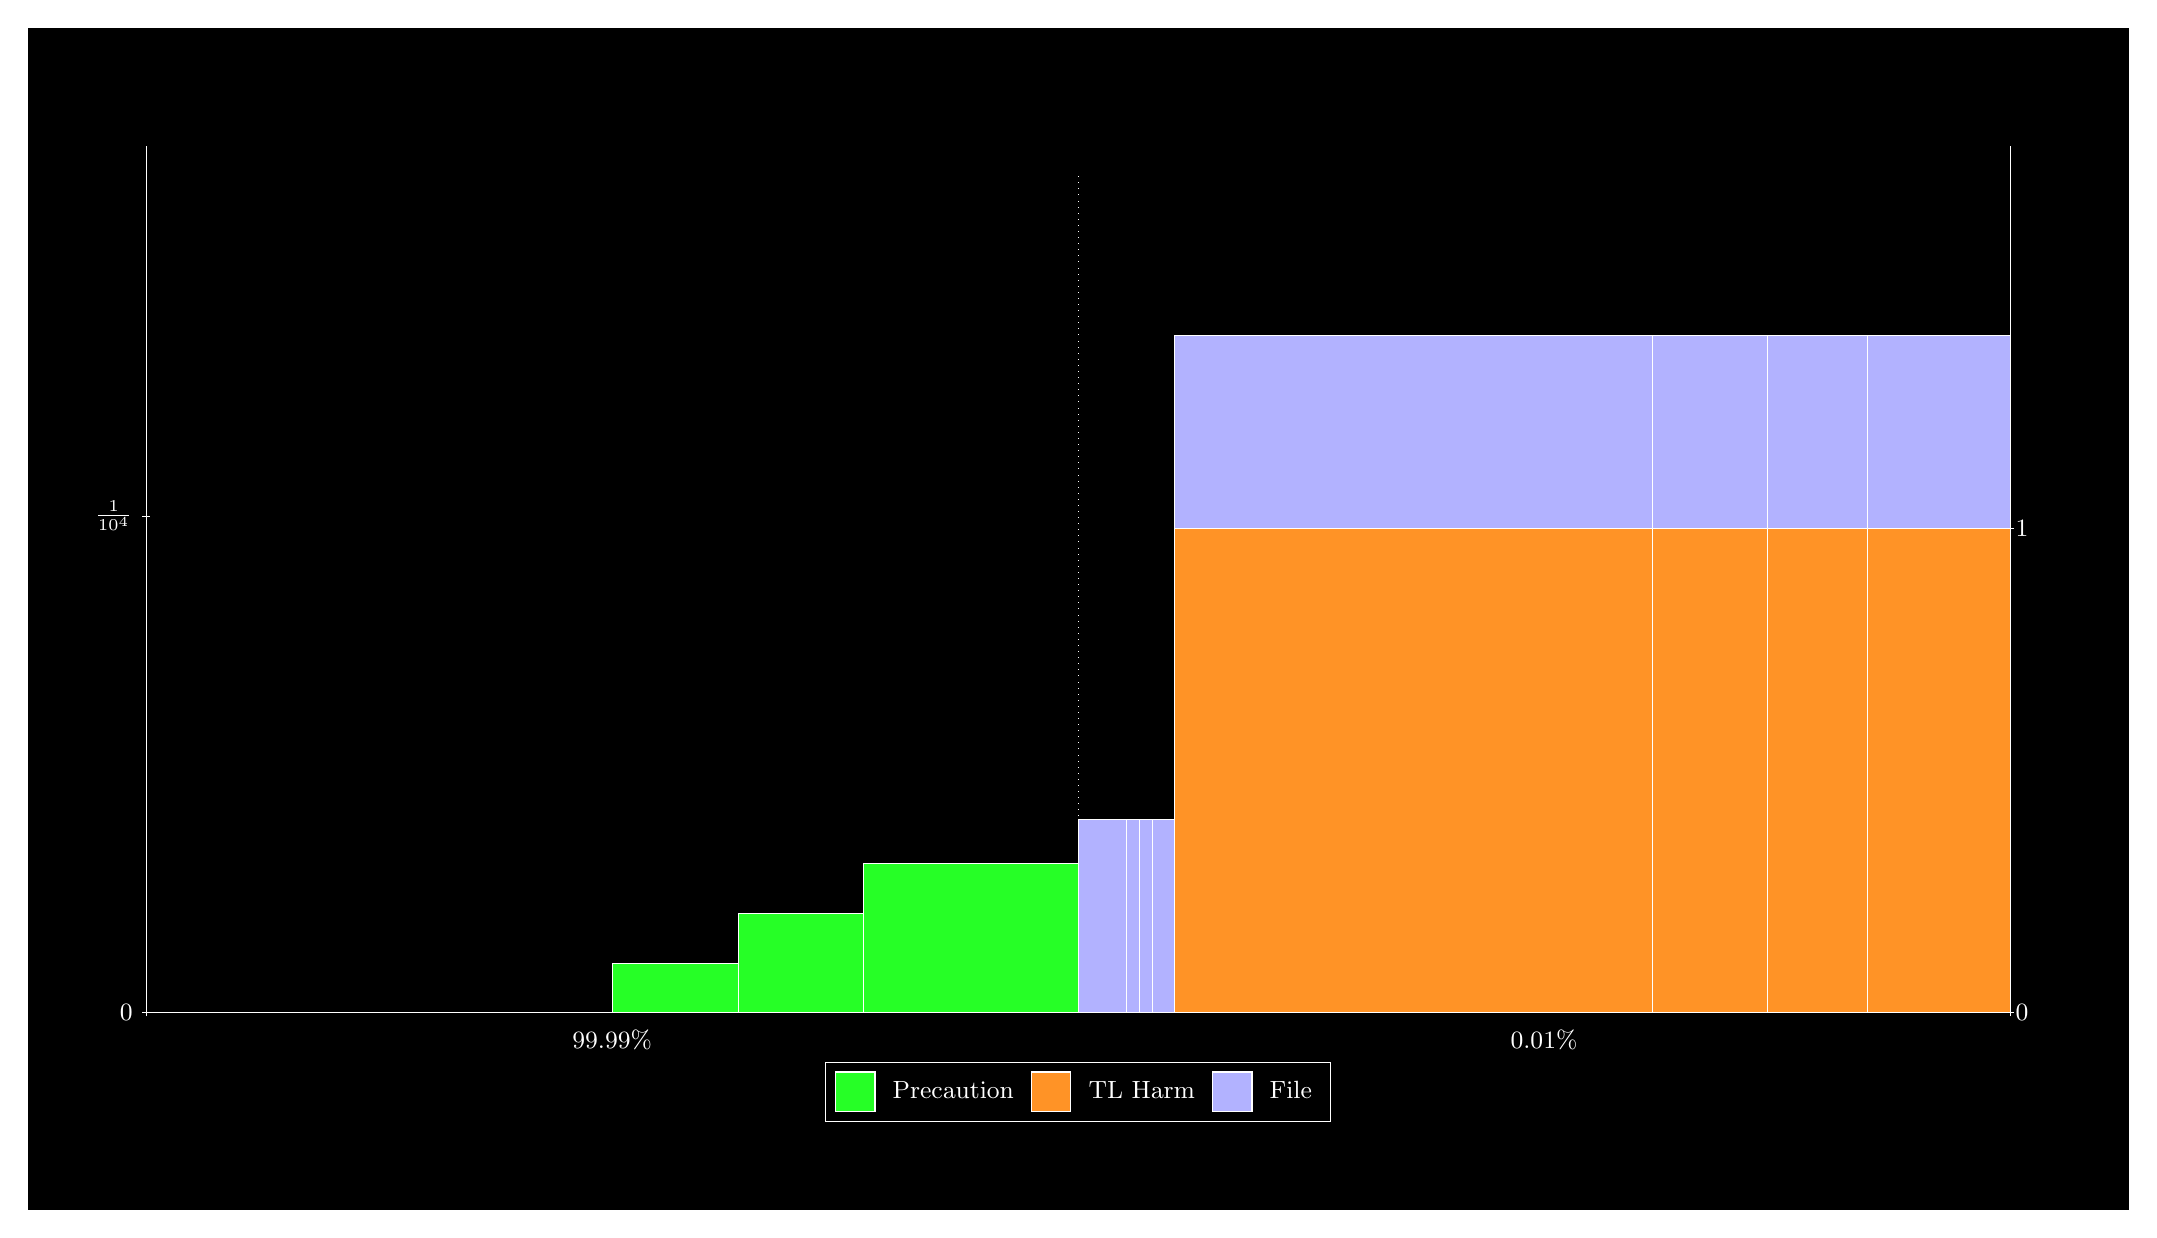
\begin{tikzpicture}
\draw[fill=black] (0,0) rectangle (26.667,15);
\draw[fill=green!85,draw=white,very thin] (7.4166,2.5) rectangle (9.0126,3.1305);
\draw[fill=green!85,draw=white,very thin] (9.0126,2.5) rectangle (10.611,3.7611);
\draw[fill=green!85,draw=white,very thin] (10.611,2.5) rectangle (13.333,4.3916);
\draw[fill=blue!30,draw=white,very thin] (13.333,2.5) rectangle (13.94,4.9575);
\draw[fill=green!85,draw=white,very thin] (13.94,2.5) rectangle (14.104,2.5001);
\draw[fill=blue!30,draw=white,very thin] (13.94,2.5001) rectangle (14.104,4.9576);
\draw[fill=green!85,draw=white,very thin] (14.104,2.5) rectangle (14.269,2.5001);
\draw[fill=blue!30,draw=white,very thin] (14.104,2.5001) rectangle (14.269,4.9577);
\draw[fill=green!85,draw=white,very thin] (14.269,2.5) rectangle (14.549,2.5002);
\draw[fill=blue!30,draw=white,very thin] (14.269,2.5002) rectangle (14.549,4.9577);
\draw[fill=orange!85,draw=white,very thin] (14.549,2.5) rectangle (20.622,8.6439);
\draw[fill=blue!30,draw=white,very thin] (14.549,8.6439) rectangle (20.622,11.101);
\draw[fill=green!85,draw=white,very thin] (20.622,2.5) rectangle (22.082,2.5001);
\draw[fill=orange!85,draw=white,very thin] (20.622,2.5001) rectangle (22.082,8.6439);
\draw[fill=blue!30,draw=white,very thin] (20.622,8.6439) rectangle (22.082,11.101);
\draw[fill=green!85,draw=white,very thin] (22.082,2.5) rectangle (23.352,2.5001);
\draw[fill=orange!85,draw=white,very thin] (22.082,2.5001) rectangle (23.352,8.644);
\draw[fill=blue!30,draw=white,very thin] (22.082,8.644) rectangle (23.352,11.102);
\draw[fill=green!85,draw=white,very thin] (23.352,2.5) rectangle (25.167,2.5002);
\draw[fill=orange!85,draw=white,very thin] (23.352,2.5002) rectangle (25.167,8.644);
\draw[fill=blue!30,draw=white,very thin] (23.352,8.644) rectangle (25.167,11.102);
\draw[white,very thin] (1.5,2.5) -- (1.5,13.5);
\draw[white,very thin] (1.45,2.5) -- (1.55,2.5);
\node[font=\small,text=white, anchor=east] at (1.45, 2.5) {0};
\draw[white,very thin] (1.45,8.8055) -- (1.55,8.8055);
\node[font=\small,text=white, anchor=east] at (1.45, 8.8055) {$\frac{1}{10^{4}}$};

\draw[white,dotted,very thin] (13.333,2.83) -- (13.333,13.17);
\draw[white,very thin] (25.167,2.5) -- (25.167,13.5);
\draw[white,very thin] (25.117,2.5) -- (25.217,2.5);
\node[font=\small,text=white, anchor=west] at (25.117, 2.5) {0};
\draw[white,very thin] (25.117,8.6439) -- (25.217,8.6439);
\node[font=\small,text=white, anchor=west] at (25.117, 8.6439) {1};

\draw[white,very thin] (1.5,2.5) -- (25.167,2.5);
\draw[white,very thin] (1.5,2.45) -- (1.5,2.55);
\node[font=\small,text=white, anchor=north] at (1.5, 2.45) {};
\draw[white,very thin] (25.167,2.45) -- (25.167,2.55);
\node[font=\small,text=white, anchor=north] at (25.167, 2.45) {};

\node[font=\small,text=white,anchor=south] at (7.4167, 1.9) {99.99\%};
\node[font=\small,text=white,anchor=south] at (19.25, 1.9) {0.01\%};
\draw (13.3333,2.5) node (B) {};
\begin{scope}[align=center]
\matrix[scale=0.5,draw=white,below=0.5cm of B,nodes={draw},column sep=0.1cm]{
\node[rectangle,draw,minimum width=0.5cm,minimum height=0.5cm,fill=green!85]{}; & \node[draw=none,font=\small,text=white]{Precaution}; &
\node[rectangle,draw,minimum width=0.5cm,minimum height=0.5cm,fill=orange!85]{}; & \node[draw=none,font=\small,text=white]{TL Harm}; &
\node[rectangle,draw,minimum width=0.5cm,minimum height=0.5cm,fill=blue!30]{}; & \node[draw=none,font=\small,text=white]{File}; \\\\
};\end{scope}

\end{tikzpicture}
\end{document}